\chapter{Architectural design}
\label{chap:chapter3}

\section{Case: Vimond Media Solution}
Vimond Media Solution \cite{bib1}, the company at whitch this thesis project was carried out,  is an OTT (Over-the-top) services provider company headquartered in Bergen, Norway. Having customers spread around the world, Vimond is one of the leader in the streaming media market. They provide for a suite of software application called Vimond Media Platform which helps content owners, broadcasters and distributors to manage their online video services. It provides top features such as Rest API, multi-tenancy support, multi-language metadata and much more.

\subsection{Vimond current architecture}

Vimond architecture (figure \ref{vimond-1}) is based of a set of microservices communicating with each other via a publish-subscribe module implemented with Apache Kafka. Using a microservices-based architecture improves modularity and scalability of the whole platform. Content providers interact with the platform with a component called Vimond Control Center, which allows them to ingest, manage and distribute their assets. End users instead, access those assets via an API abstraction over the microservices, after being authenticated with O-Auth protocol. At the moment, relevant actions such as subscription purchase or asset playing performed by end-users are just stored into Cassandra and Oracle databases and used only when needed, for instance when customers request usage reports. What it missing is an independent module for gathering and analyzing these data, possibly in real-time with support for historical data. Lambda architecture seems perfect for defining such a module and in the rest of this chapter we are going to show and describe the proposed framework for this problem.

\begin{sidewaysfigure}
\centering

        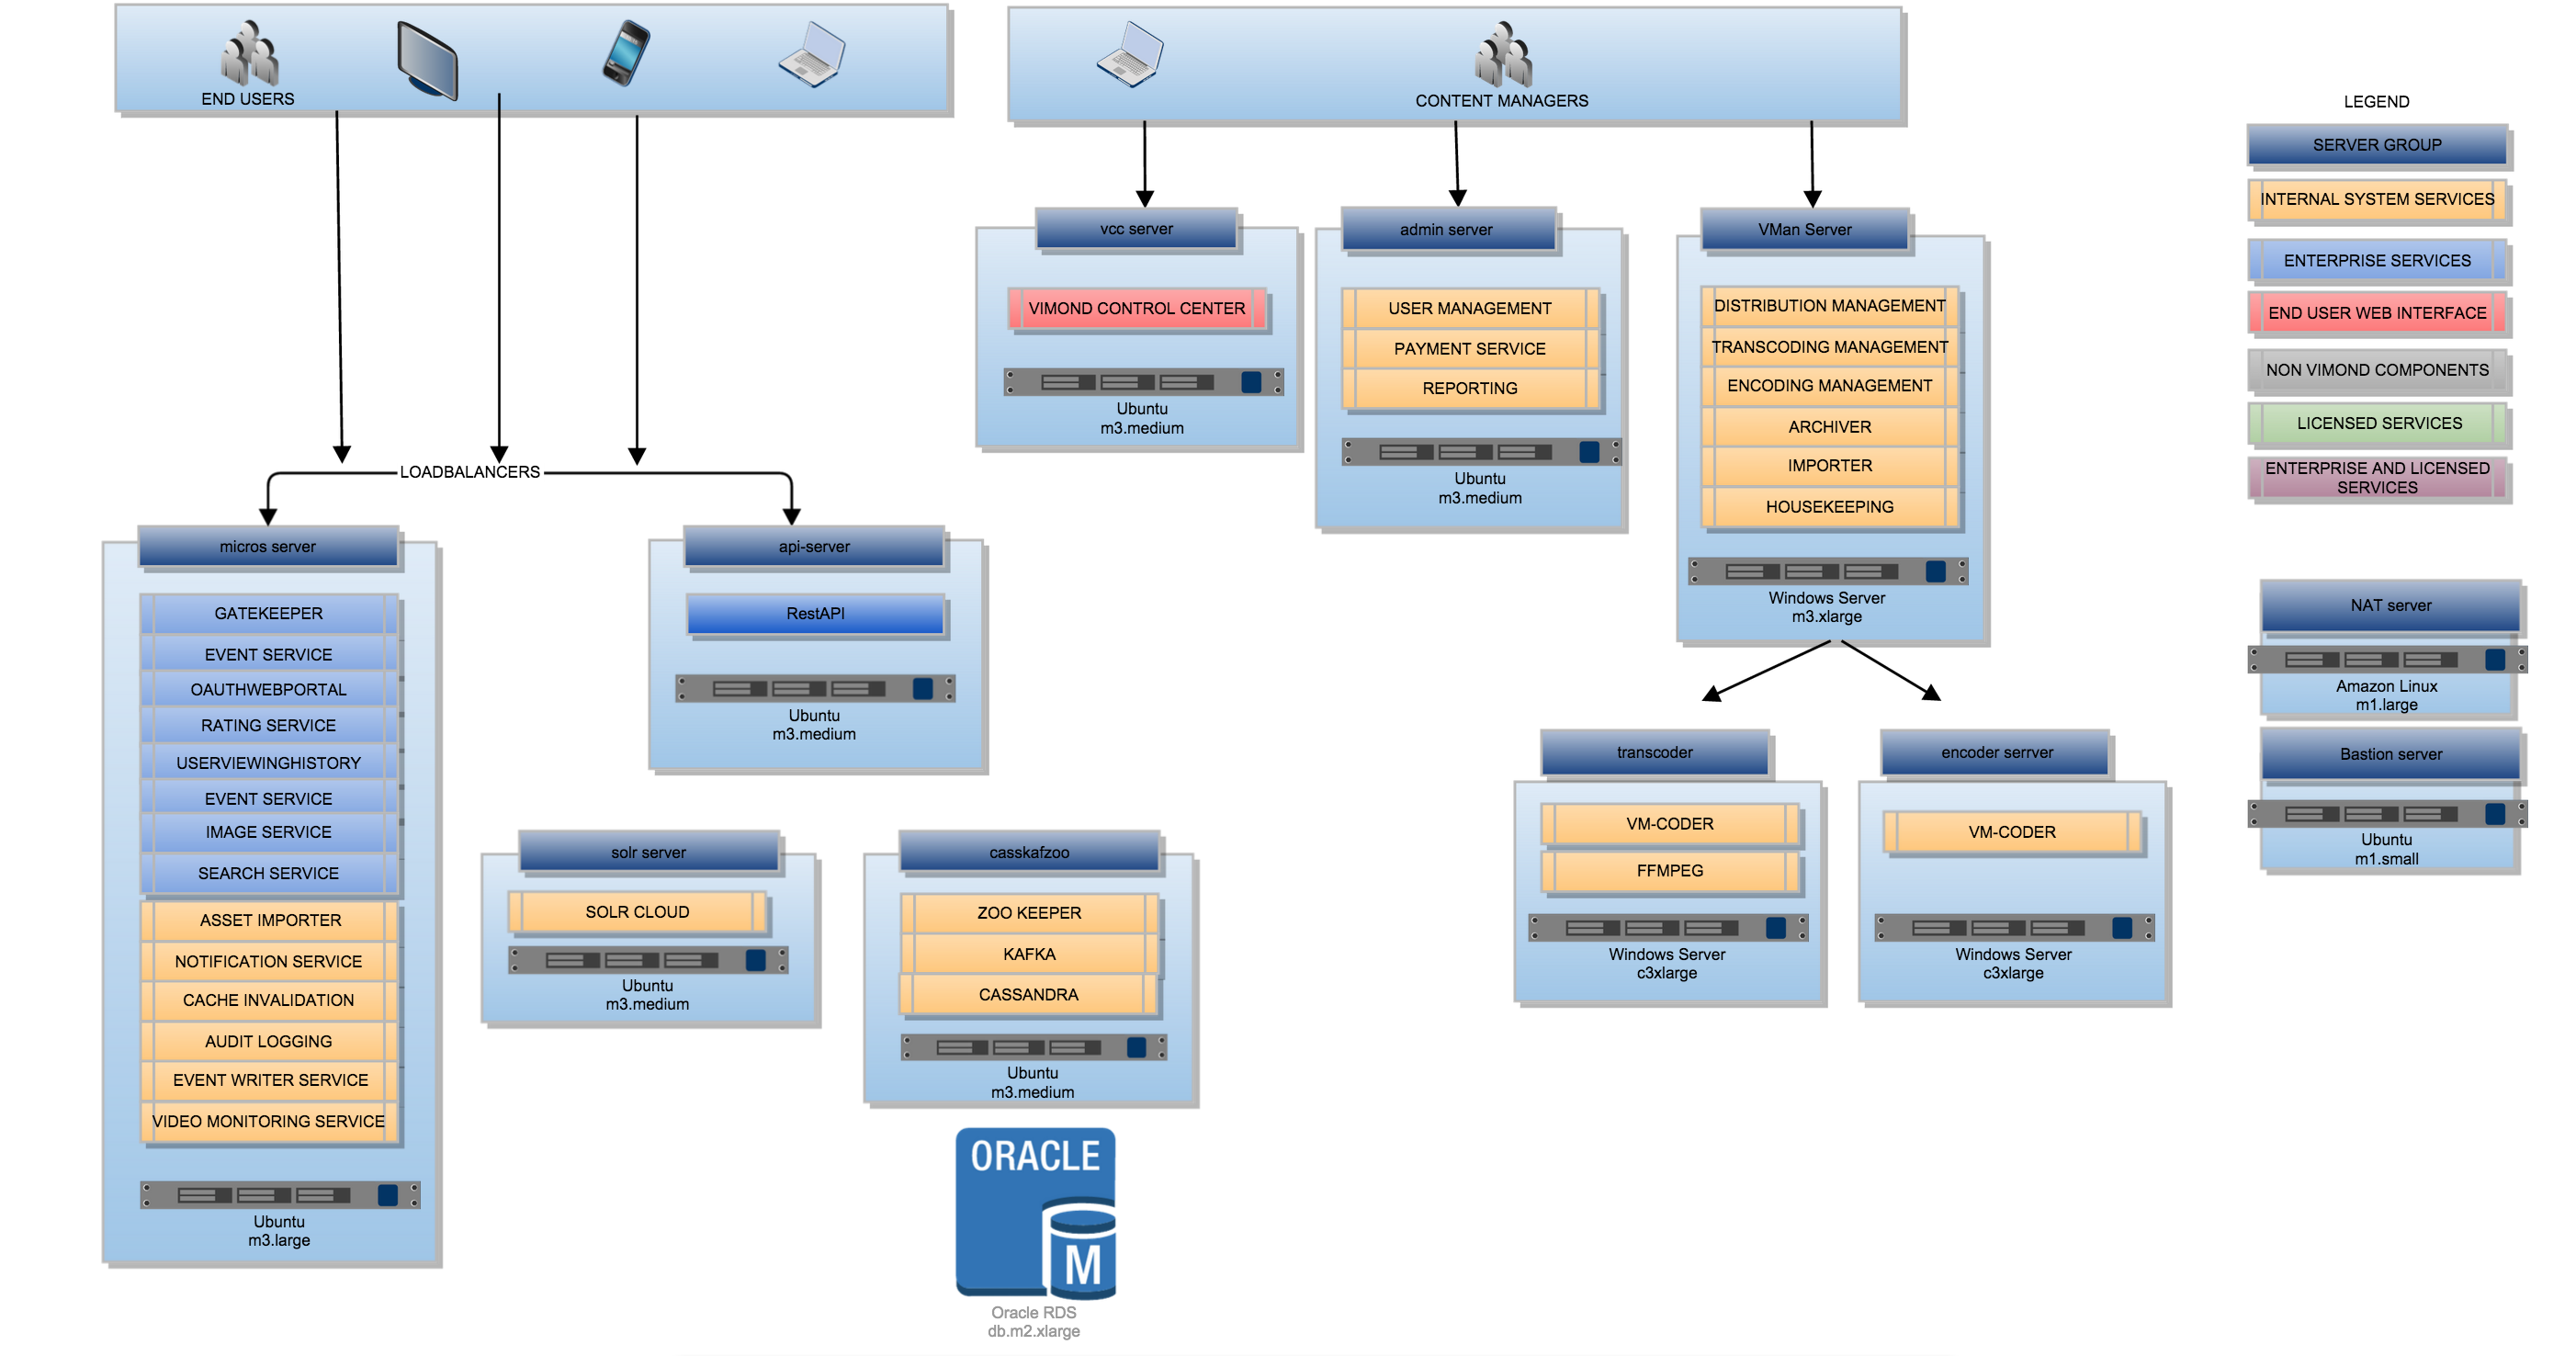
\includegraphics[width=20cm]{imgs/vimond-architecture}
\caption[Vimond architecture example]{Example of Vimond production envirovment.}
        \label{vimond-1}
\end{sidewaysfigure}

\section{Proposed solution}
The proposed solution is meant to be a prof of concept of Lambda architecture, rather then an effective production-ready system. It aims to improve the theoretical idea by simplifying it where there are the majority of problems (i.e. the complexity), resulting still in a three layer architectural pattern. For the rest of the report we will refer to this model as VimondAnalytics.\\
The main simplification comes when dealing with intermediate views. According to the original Lambda architecture pattern, each processing layer produces intermediate views to be merged into global ones in the serving layer. The model we are going to propose avoid storing intermediate views in different databases, data instead are ingested directly in the serving layer. The purpose of the latter is similar to the original one as it has to merge data coming from the two different processing layers, but now, instead of merging views, it merges raw data coming from the real-layer and aggregated ones from the batch layer. The simplification is hence obvious: there is no need anymore for different storage solutions which have different requirements and therefore different problems. All the complexity is moved to the serving layer while the real-time and the batch layer fulfill only to processing requirements. \\

\begin{figure}[h]
        \makebox[\textwidth][c]
        {
        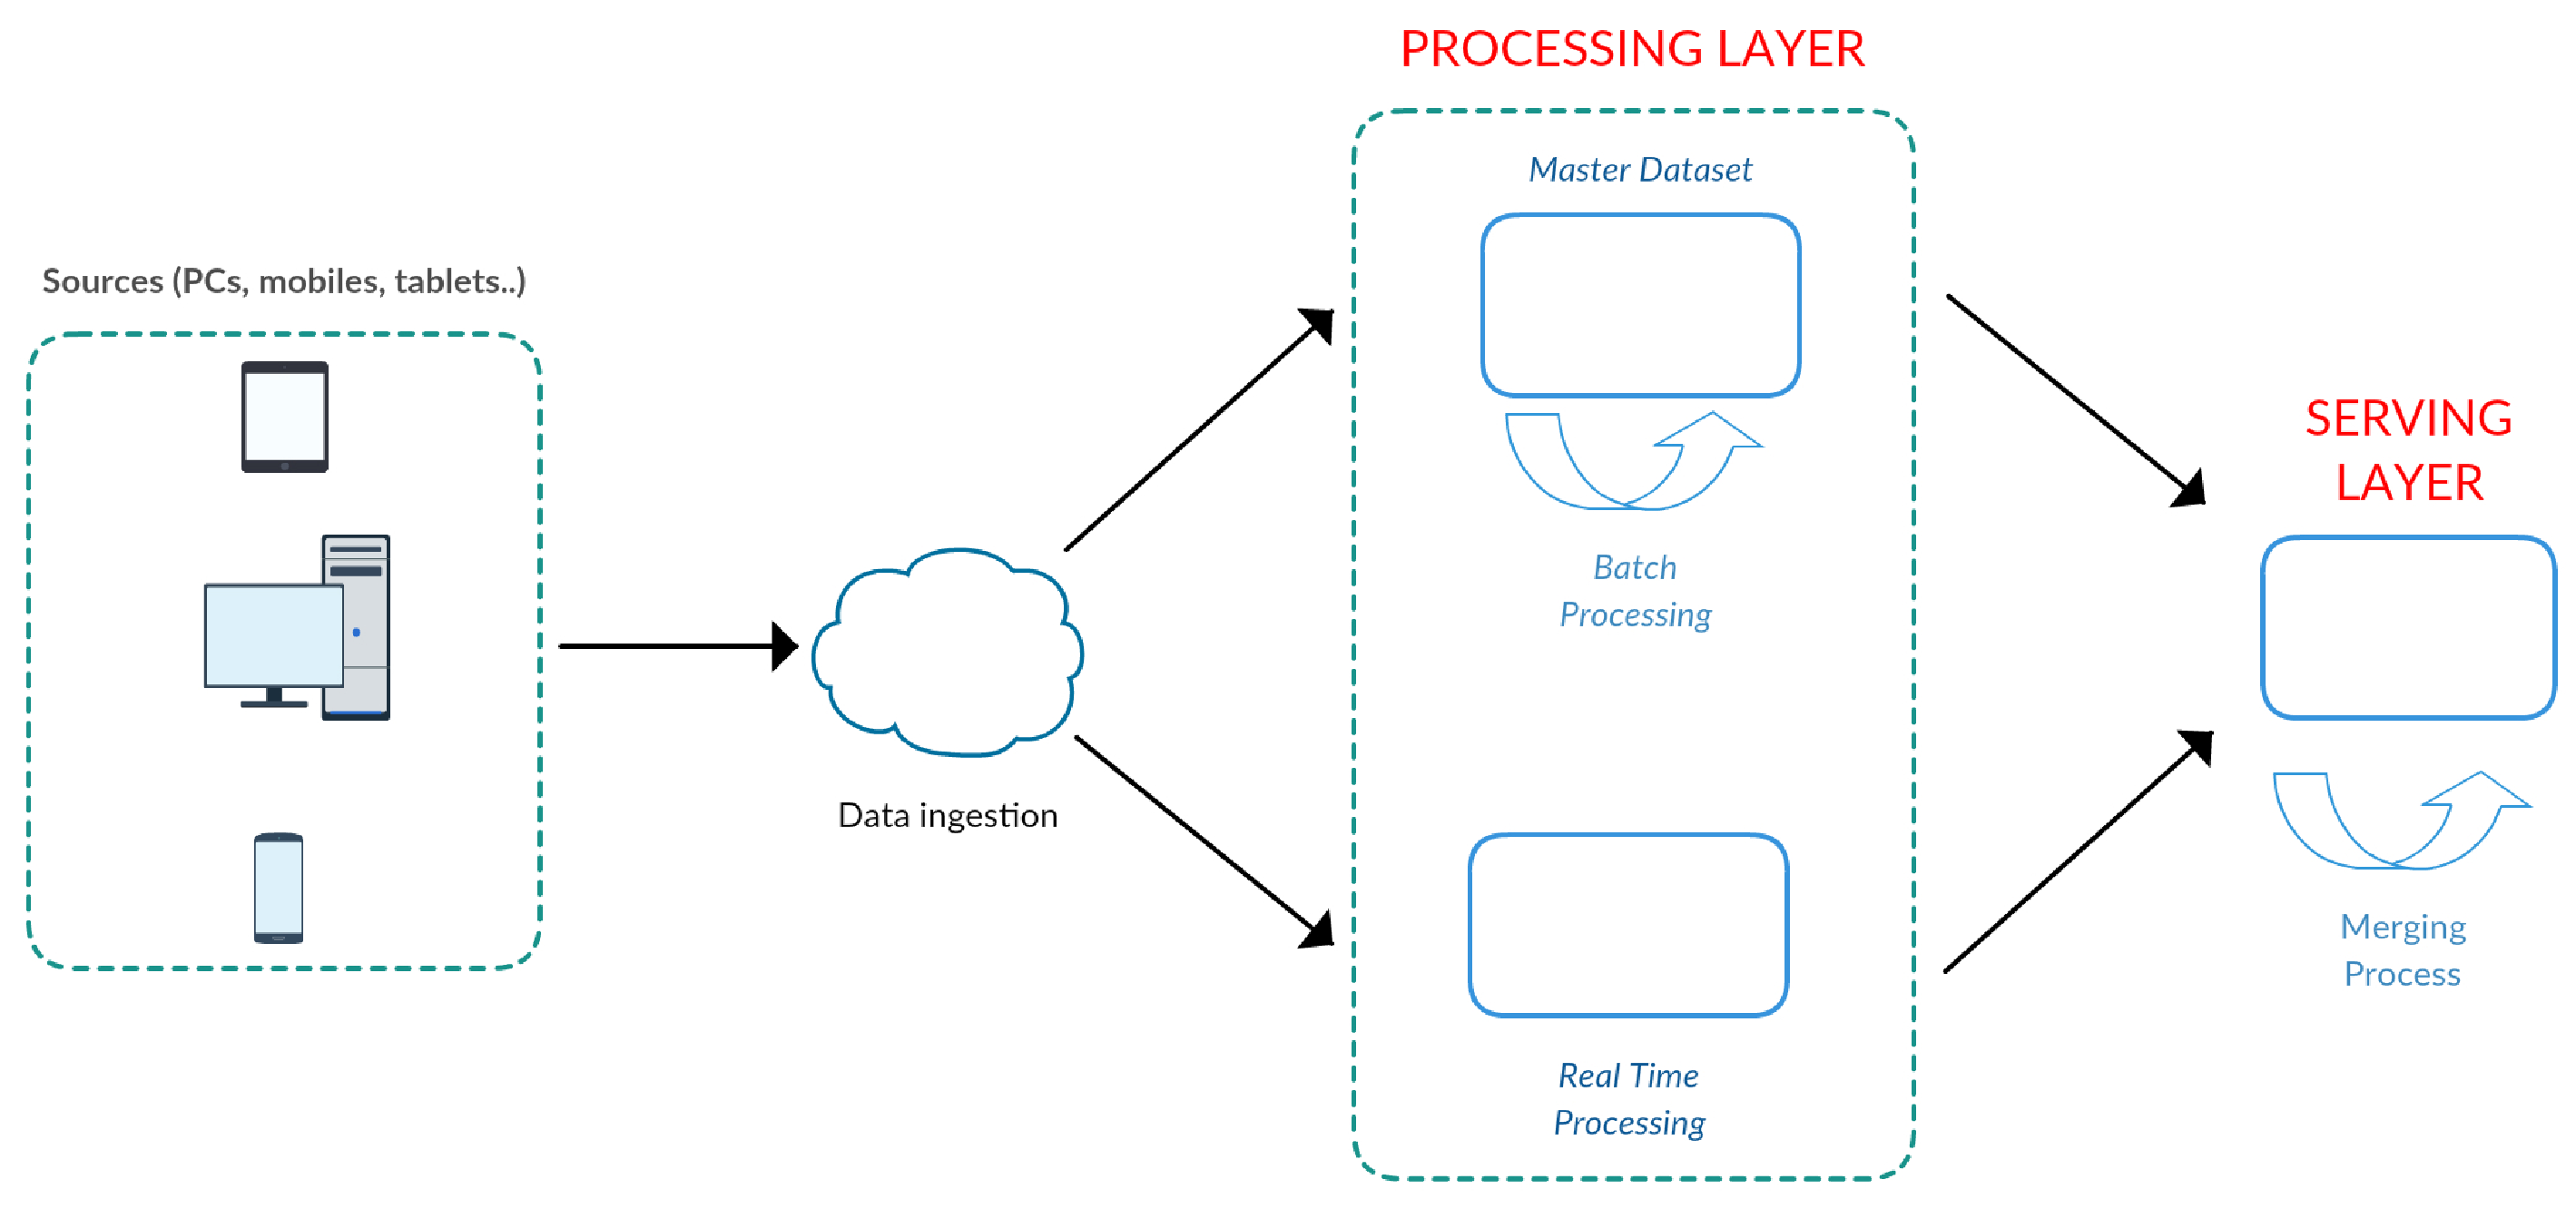
\includegraphics[width=17cm]{imgs/vimondAnalytics}
        }
\caption[VimondAnalytics architecture]{VimondAnalytics architecture}
        \label{vimondAnalytics-1}
\end{figure}

The final architecture is again a composition of several layers. Data come into the system through a \textit{data ingestion} layer, implemented with a publish/subscribe architecture. The \textit{real-time layer} gets data from the data ingestion and after few processing steps, stores them in the serving layer. The \textit{batch layer} stores data in a data lake structure and runs aggregation processes for obtaining compact (and shorter) views out of them, which will be eventually stored as well in the serving layer. The latter aggregates raw data and merges them with the batch ones in order to answer to end-users queries.\\
The rest of the chapter describes each separate layer of the model above briefly introduced.

\subsection{Data ingestion}
Data ingestion layer represents the entry point of the system, where input data are managed and replicated into the batch and the real-time layer. Apache Kafka fits perfectly into this role, as is it handles different consumers and has them fetching messages from different points on the same dataset, according to their capability. \\
In order to get the whole system working we need a data source. Normally artificial dataset can be used for a prof of concept validation but we preferred to use a real one. Vimond provides TV2 Norway with services for its online streaming platform called \textit{TV2 Sumo}. Data used in this project come from that platform and refer to a  player playback functionality which allows a user to resume the stream of an asset when it closes the browser window and wants to re-play from the last point.\\

\subsection{Real time layer}
The real-time layer of this model is very simple, its purpose is to forward data from the data ingestion part to the serving layer after processing them. Differently from the original approach, it does not have to generate any aggregation or storing data on an intermediate database. A possible process executed in this layer could be data augmentation, like IP translation into location and coordinates or user agent breaking into browser and operative system version. Neither an incremental nor a recomputation algoritm is used: augmented data are just written on the serving layer. A typical example of data forwarded by the real time layer could be: 
\begin{listing}
\begin{minted}[frame=single,
               framesep=3mm,
               linenos=true,
               xleftmargin=21pt,
               tabsize=4]{js}
{     
    "eventType": "click"
    "userId" : "12345",
    "targetURL" : "http://www.mywebsite.com/mypage.html"
    "timestamp": "2015-09-06-19:54:00"
}
\end{minted}
\caption{RealTime data example} 
\label{realtimedata-example}
\end{listing}

Apache Storm has been used for implementing this layer as it provides the features we need. No message guarantee policy is required, we are not interested in having a strong consistency level, data need to be moved as fast as possible and a certain degree of inaccuracy is tolerated. Anyway, real-time processing frameworks such as Storm allow to implement an \textit{at-least-once} message processing instead of \textit{at-most-once} where messages loss is possible. According to the use cases of the current scenario, it is possible to switch to the semantic needed.

\subsection{Batch layer}
\label{batch-layer1}
The batch layer is organized in two parts. First data are fetched from the data ingestion layer and saved into a data lake, then they are analyzed and aggregated according to the output views.\\
In order to improve the performances of the fetching process, data are stored in the data lake in batches and two mode of doing it were implemented: 
\begin{itemize}
\item \textbf{unreliable}: the offset for a message is committed after it has been read from the data ingestion layer. This implies that, if the process crashes or fail to write the message on the data lake, the message is lost. In addition, if messages are processed in batch, in case of crash of the process, all the batch is lost. This approach implements a \textit{at-most-once} message delivery semantic.
\item \textbf{reliable}: the offset is committed after a batch of messages is written successfully on the data lake. In case of crash of the process, the one who takes over is going to read from the last committed offeset which represent the latest checkpoint. In case of crash of the process after writing the  messages but before committing the offeset, data will be written twice. This approach implements a \textit{at-least-once} message delivery semantic.
\end{itemize}
Data lake is implemented through Hadoop HDFS. As explained in the previous chapter, HDFS implements an abstraction over a distributed data storage such that classic filesystem operations are possible. Data written into the data lake are organized in a time-folders structure: the dataset is a hierarchy of folders where at the top there are the ones representing days, the second level is for the hours of a particular day and the third is for the division of the hour in intervals. It is possible to divide an hour or a day in several intervals but partitions bigger than a day were not implemented. When a new datum needs to be written in the dataset, it goes to the corresponding folder according to its timestamp. For instance,  let assume a partition criteria of 15 minutes: this means that every folder representing an hour contains 4 sub-folders representing the minutes intervals (00-14, 15-29, 30-44, 45-59). The figure \ref{datalake-1} explains where data are actually written in this scenario, according to their timestamp.

\begin{figure}[h]
        \centering
        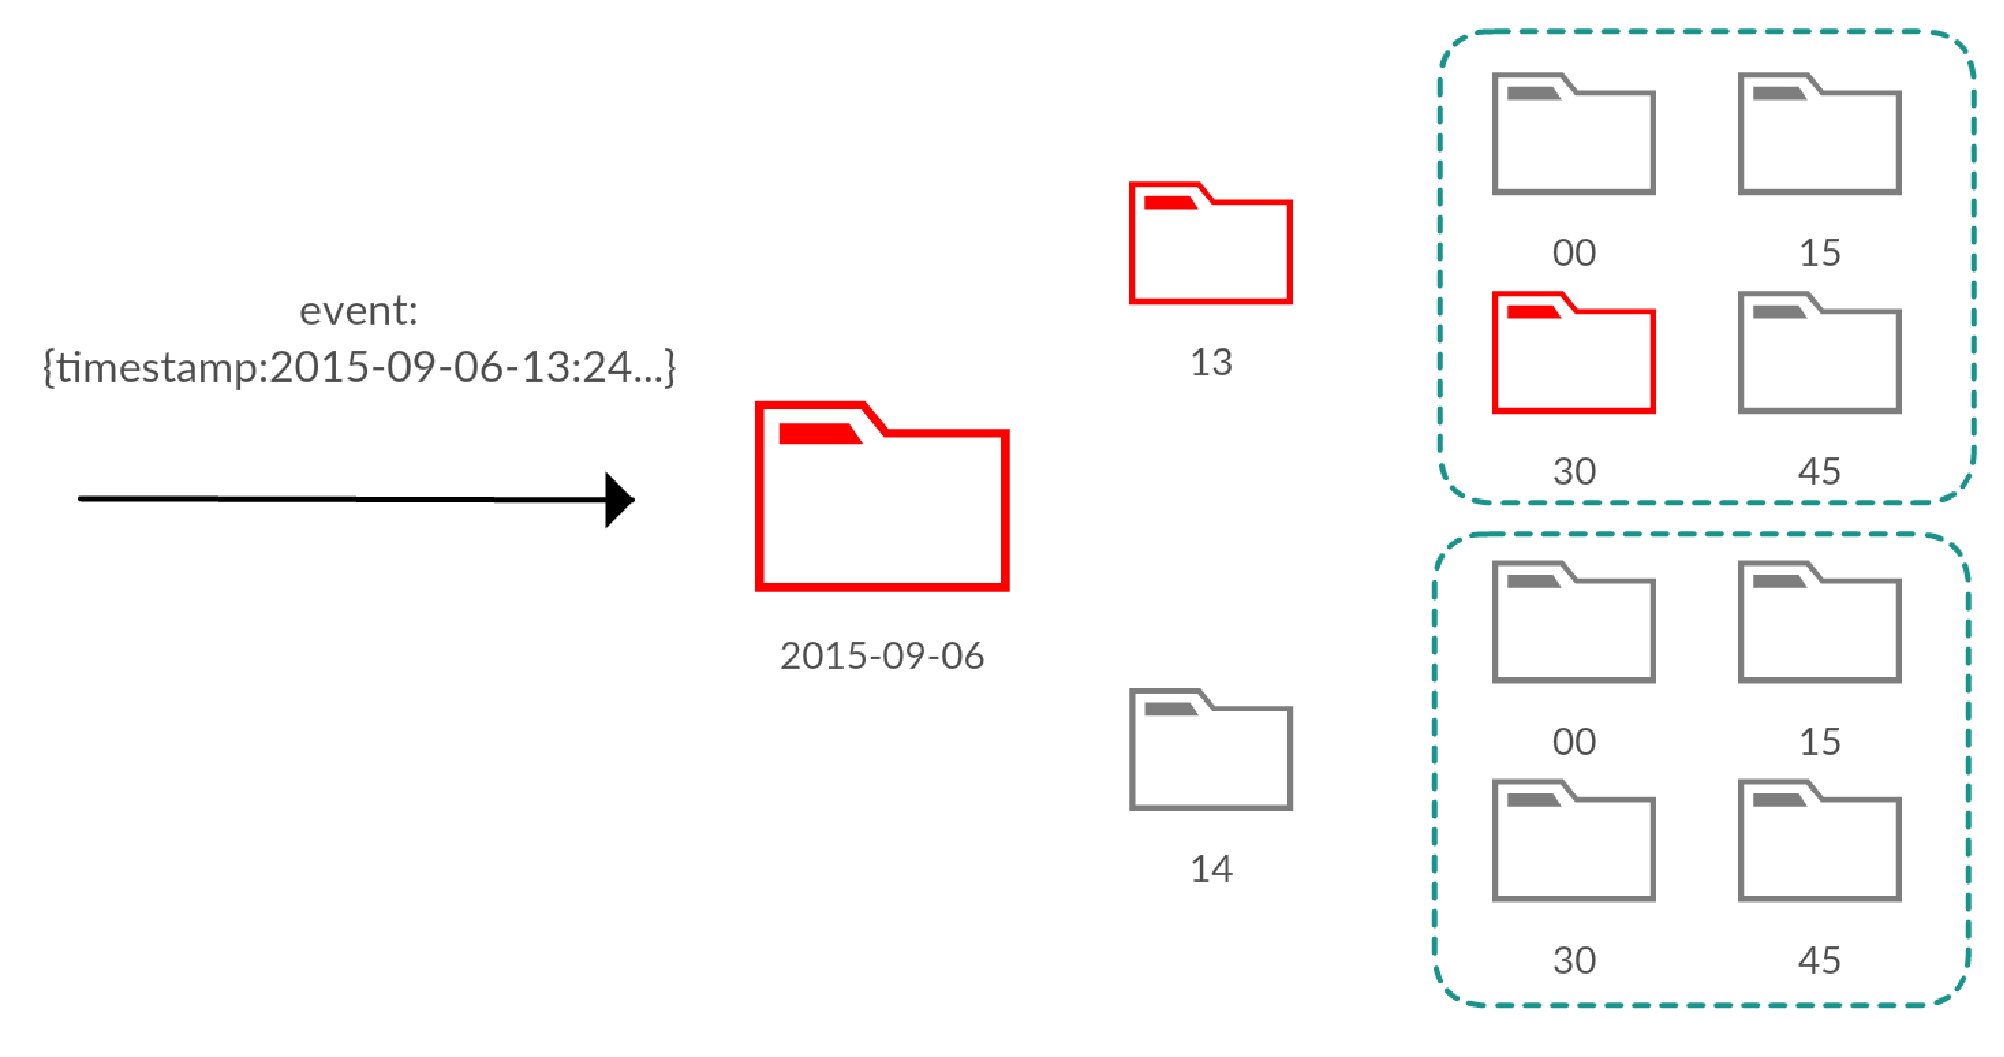
\includegraphics[width=12cm]{imgs/datasetStructure}
\caption[Data lake structure]{Time folder structure: an event is saved in the corresponding folder, according to its timestamp.}
        \label{datalake-1}
\end{figure}

While new data are ingested into the data lake, the batch layer is responsible to execute aggregation processes on the historical ones. Each of these processes takes in input data contained inside a specific folder, which changes over the different executions, and produces as output a set of events representing aggregated data and they are stored directly into the serving layer, without the use of an intermediate database. A typical example of a datum generated by this layer could be:
\begin{listing}
\begin{minted}[frame=single,
               framesep=3mm,
               linenos=true,
               xleftmargin=21pt,
               tabsize=4]{js}
{     
    "eventType": "click"
    "targetURL" : "http://www.mywebsite.com/mypage.html"
    "counter": 100
    "timestamp": "2015-09-06-19:54:00"
}
\end{minted}
\caption{Batch layer data example} 
\label{batchlayer-example}
\end{listing}

An incremental approach can be used, but this model has been thought for a recomputational one over the different data subsets. The different batch views produced at each execution can be aggregated with each others in the serving layer. While this approach simplifies a lot the whole aggregation processes, it has limitations in the type of results it can produce as explained in the last subsection of this chapter.\\
Finally, after a batch window of data has been processed, according to the principles of Lambda architecture, real-time data included in that time window are no longer needed as we have an aggregated version, much smaller and faster to query. It is a duty of this layer ensuring that, after the succesful completion of a batch process, the corresponding real-time data are deleted. In this way, all the approximation made by the real-time layer are eventually corrected by the batch views.

\subsection{Serving layer}
The serving layer of VimondAnalytics presents the biggest differences with the original idea proposed by Lambda architecture. As said in the previous chapter, the serving layer should index the batch views and merge them with the real-time ones. Here instead, we don't have anymore the concept of intermediate views, but only final ones are presented to end-users. For this purpose, it is needed a solution which provides storage and aggregation functionalities.\\
Two kind of data are written into the serving layer:
\begin{itemize}
\item data coming from the real-time layer
\item aggregated data coming from the batch layer. 
\end{itemize}
According to the data example provided in the previous sections, a serving view regarding the count of clicks for a particular web page merges all the real-time data for that webpage with the ones generate from the batch layer, according to the timeframe requested by the query. If the serving layer uses JSON syntax as well, then an output result could be the one proposed in figure \ref{servinglayer-example}.
\begin{listing}
\begin{minted}[frame=single,
               framesep=3mm,
               linenos=true,
               xleftmargin=21pt,
               tabsize=4]{js}
{     
    "eventType": "click"
    "targetURL" : "http://www.mywebsite.com/mypage.html"
    "counter": 200
    "from": "2015-09-06-19:00:00"
    "to": "2015-09-06-20:00:00"
}
\end{minted}
\caption{Serving Layer data example} 
\label{servinglayer-example}
\end{listing}
Elasticsearch was used for implementing this layer. We are not interested in the full-text search engine but we exploited mostly its aggregation functionalities on the documents stored into it. 
\subsection{Considerations}
\label{chap3:consideration}
In this chapter we presented a Lambda architecture based model for big data analytics. The idea behind this model is the simplification of the theoretical one, removing intermediate views and then complexity to the whole system and computing final views in the serving layer, as a combination of raw data and batch results.\\
Concerning the batch layer, looking at the data in time windows causes limitations in the type of results that can be overall computed. Let assume to have two consecutive batch windows of data, created by a time partitioning structure as explained in the section \ref{batch-layer1}. The different results calculated on each window are then stored in the serving layer and aggregated with each others if a query wants to extract data from a time interval containing both of them. Hence, we need to ensure that the aggregated results are consistent among all the different batches, which is, given two partitions \textit{A} and \textit{B} and an aggregation function \textit{f}, the following equation $f(A) + f(B) = f(A+B)$ must hold. For all the other cases where it does not hold, an incremental approach is needed. Example of consistent views are generated by unique events over the time, like a purchase or a content rating. \\
Other limitations of this approach are inherited from the Lambda architecture one: it is not possible to query the system for a time interval shorter than the batch time window. The smaller the granularity, the greater the accuracy of the query, but computing batch jobs more frequently might not be the best option in terms of efficiency, even if applied on a smaller subset of data.\\
The applicability of this framework lies on the use cases where a normal query would investigate what happened in a fixed time span in the past, corresponding to one or more batch windows (for instance, recalling the previous example, the number of clicks for a webpage from 10 am to 12 am, assuming a 30 minutes batch interval), or a real-time overview over all the historical data saved in the serving layer.